\documentclass[sigconf,nonacm]{acmart}

\usepackage{booktabs}
\usepackage{graphicx}
\usepackage{listings}
\usepackage{xcolor}
\usepackage{enumitem}
\usepackage{microtype}
\usepackage{float}
\usepackage{xspace}
\usepackage{pifont}
\usepackage{makecell}
\usepackage{colortbl}

\newcommand{\system}{\textsc{Aegis}\xspace}
\newcommand{\bench}{\textsc{ToolGuard-Bench}\xspace}
\newcommand{\cmark}{{\color{green!60!black}\ding{51}}}
\newcommand{\xmark}{{\color{red!70!black}\ding{55}}}

\lstset{
  basicstyle=\footnotesize\ttfamily,
  frame=single,
  rulecolor=\color{gray!50},
  backgroundcolor=\color{gray!5},
  keywordstyle=\color{blue!70!black},
  stringstyle=\color{green!50!black},
  commentstyle=\color{gray},
  breaklines=true,
  showstringspaces=false,
  aboveskip=5pt,
  belowskip=5pt,
  xleftmargin=3pt,
  xrightmargin=3pt,
  numbers=none,
}

%% ACM metadata — fill in final camera-ready values
\settopmatter{printacmref=true, printfolios=true}

\begin{document}

\acmConference[CAIS '26]{ACM Conference on AI Safety}{2026}{}

\title{AEGIS: No Tool Call Left Unchecked --- A Pre-Execution Firewall
for AI Agents, and What It Actually Catches}

\author{Aojie Yuan}
\affiliation{%
  \institution{University of Southern California}
  \city{Los Angeles}
  \state{California}
  \country{USA}
}
\email{aojieyua@usc.edu}

\author{Zhiyuan Su}
\affiliation{%
  \institution{University of California, Davis}
  \city{Davis}
  \state{California}
  \country{USA}
}
\email{azysu@ucdavis.edu}

\author{Yue Zhao}
\affiliation{%
  \institution{University of Southern California}
  \city{Los Angeles}
  \state{California}
  \country{USA}
}
\email{yue.z@usc.edu}

\begin{abstract}
AI agents increasingly execute tool calls---database queries, shell commands, file operations, and HTTP requests---yet most agent frameworks forward these calls to execution with no pre-execution mediation.
We present \system, a pre-execution firewall and audit layer for AI agents.\footnote{Open-source (MIT). Code: \url{https://github.com/Justin0504/Aegis}.}
\system interposes on the tool-execution path with a three-layer cost-aware cascade, supports 14 agent frameworks across Python, JavaScript, and Go, and provides tamper-evident auditing, human-in-the-loop approval, and a compliance dashboard.

This version reports a substantially revised evaluation, and revises the conclusions of our earlier one.
Auditing the benchmark we had used to validate the system, we find it does not measure what it claims: of 5{,}525 records, 144 carry no arguments to inspect and 5{,}195 are exact duplicates, and the malicious records encode their own label in an argument key present in 3{,}196/3{,}196 InjecAgent attacks and 0/2{,}108 benign calls---so that \textbf{argument character count alone separates the classes at AUC 0.918}, and fifteen surface features reach 0.996.
Effective sample size is \textbf{186 unique evaluable calls}, of which only \textbf{21 are benign}: the 0.09\% false-positive rate we previously reported is not estimable from 21 items, whose smallest non-zero value is 4.8\%.
The cause is structural: the corpora such benchmarks are built from are agent-\emph{execution} suites that contain no concrete attacker tool call, so converting them to static per-call data requires fabricating one.
We therefore rebuild by running an agent, recording what a live model emits under injection.
A matched control arm isolates the effect---attack success \textbf{95.1\%} versus \textbf{0.3\%}, risk ratio 334.

On the corrected data our own headline collapses. \system's 22 detection patterns fire on \textbf{0.4\%} of real attack calls, because a successful indirect injection produces a syntactically innocent call such as \texttt{ViewSavedPaymentMethods(\{\})}; the apparent 84.4\% block rate is schema validation, which also rejects 73.9\% of legitimate traffic.
Payload inspection is the wrong abstraction: what makes such a call an attack is not in the call string.
We then show what is. Replacing data provenance (which argument came from a tool) with \textbf{instruction provenance} (which turn authorised this call) reaches \textbf{AUC 0.991} against a control in which benign calls also draw on tool output, versus 0.737 for taint features and 0.687 for content, and holds at 0.933 against an attacker who shapes the call to mimic the user's own request.
Benchmark, rollout harness, audit, and provenance layer are released under MIT license.
\end{abstract}

\keywords{AI Agent Safety, Tool-Call Interception, LLM Guardrails, Runtime Compliance}

\maketitle

\begin{figure*}[t]
    \centering
    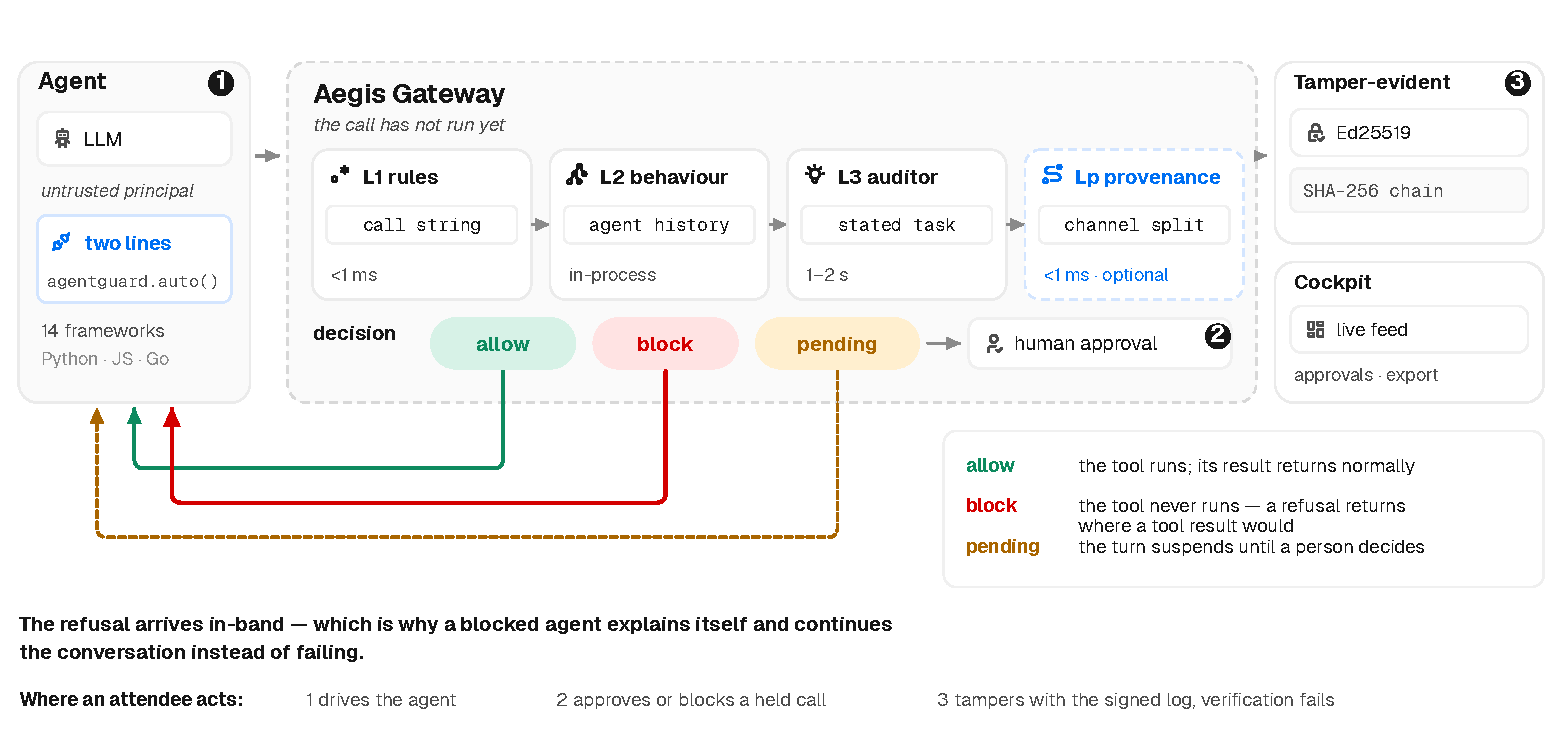
\includegraphics[width=\textwidth]{images/architecture.pdf}
    \vspace{-0.1in}
    \caption{\system on the tool-execution path. The SDK instruments 14 frameworks to intercept \texttt{tool\_use} before execution. Cascade layers are ordered by \emph{observation scope}, not only by cost: L1 sees the call string, L2 a 15-dim surface encoding, L$_\mathrm{p}$ the trusted/untrusted channel split, L3 the full context. Reported numbers are measured on the instantiated corpus of \S\ref{sec:instantiate}, not on the withdrawn benchmark of \S\ref{sec:audit}. Every decision is Ed25519-signed and chained.}
    \vspace{-0.1in}
    \label{fig:architecture}
\end{figure*}

\section{Introduction}
\label{sec:intro}

AI agents do not only generate text; they take actions.
ReAct~\cite{yao2023react} showed that LLMs can interleave reasoning with tool invocations, and modern frameworks such as LangChain~\cite{langchain2023}, CrewAI~\cite{crewai2024}, and LlamaIndex~\cite{llamaindex2024} have made tool-augmented agents widely accessible.
However, these capabilities create a direct path from model output to real-world side effects---a path that can be triggered by adversarial prompt injection~\cite{greshake2023not} or hallucinated reasoning.
In most current stacks, once the model emits a tool call, the framework forwards it to execution with no pre-execution control point.

Post-execution observability platforms such as Langfuse~\cite{langfuse2024} and Arize~\cite{arize2024} can record these events, but they cannot prevent side effects before they occur.
Existing defenses sit at two extremes: rule-based layers are fast ($<$1\,ms) but brittle against unseen attack patterns, while LLM-judge layers generalize well but add seconds of latency per call.

We present \system, a pre-execution firewall that bridges this gap with a \textbf{cost-aware three-layer cascade}, and---in this version---an evaluation that revises what we previously claimed for it.

\paragraph{Why this version differs.}
An earlier version of this paper reported that the cascade blocks 99.9\% of attacks at 0.09\% false positives, outperforming every standalone LLM judge on every metric, and that a 27.2\% cross-source generalization gap motivated the cascade design.
Those numbers came from a static per-call benchmark we built ourselves, and auditing its construction shows the benchmark cannot support them (\S\ref{sec:audit}).
They are withdrawn here.
This is not a defect of one loader. The public corpora that per-call agent-security benchmarks are assembled from---InjecAgent~\cite{zhan2024injecagent} and ToolEmu~\cite{ruan2024toolemu}---are agent-\emph{execution} suites: neither ships a concrete attacker tool call, because that call exists only after an agent has read an injection and decided what to do.
Converting them to per-call data therefore requires \emph{fabricating} the call, and the fabrications in use are degenerate in a way no held-out split can detect, because the shortcut is present in every record of the class.

\paragraph{What replaces them.}
We rebuild the evaluation the only way that is sound, by running an agent and recording what it actually emits (\S\ref{sec:instantiate}), with a matched control arm that swaps the injection for length-matched neutral prose so the effect is causal rather than correlational.
On the resulting corpus the cheap layers of our own cascade do not work: pattern matching fires on 0.4\% of real attack calls (\S\ref{sec:eval}).
This is not a tuning deficiency. A successful indirect injection produces a call that is syntactically ordinary---\texttt{ViewSavedPaymentMethods(\{\})} carries no argument at all---so there is nothing in the call string for a pattern to match.
The finding generalizes beyond \system: any defense that inspects payloads is looking at the wrong object.

\paragraph{What does work.}
If the attack is not in the call, it is in the call's provenance. We distinguish \emph{data} provenance, which the literature's taint features already track, from \textbf{instruction provenance}: which turn authorised this call, and whether that turn was attacker-controlled (\S\ref{sec:prov}).
Against a benign control in which legitimate calls also draw their arguments from tool output---the control that makes the comparison honest---four instruction-provenance features reach AUC 0.991, against 0.737 for taint and 0.687 for content, and hold at 0.933 under an adaptive attacker.

\medskip\noindent Our contributions are:
\begin{enumerate}[nolistsep,leftmargin=*]
\item A \textbf{framework-agnostic interception layer} supporting 14 agent frameworks across Python, JavaScript, and Go with two-line integration, with tamper-evident auditing and human-in-the-loop approval.
\item A \textbf{forensic audit} of static per-call agent-security benchmarks, including our own, showing three independent construction failures that reduce 5{,}525 records to 186 evaluable calls---21 of them benign---and let a single surface feature reach AUC 0.947.
\item An \textbf{instantiation protocol} that rebuilds the benchmark by agent rollout, with a matched control arm establishing a causal effect (95.1\% vs 0.3\%, RR 334) and an integrity report showing no surface feature above AUC 0.585.
\item A \textbf{negative result with a mechanism}: payload inspection detects 0.4\% of real attack calls, and \textbf{instruction provenance}---a feature family not previously represented---reaches AUC 0.991 on the same data, with its adaptive failure mode measured rather than assumed.
\end{enumerate}

\section{System Overview}
\label{sec:arch}

\noindent\textbf{Threat Model.}
We treat the LLM as an \emph{untrusted component}: it may generate harmful tool calls due to indirect prompt injection~\cite{greshake2023not}, hallucinated reasoning, or jailbreak attacks. The SDK and Gateway are trusted enforcement components. \system does not defend against attacks that bypass the SDK entirely.

\subsection{SDK Layer: Transparent Tool-Call Interposition}
\label{sdk-layer}

The SDK intercepts LLM API responses via runtime instrumentation. When a response contains a \texttt{tool\_use} block, the SDK extracts the tool name and arguments, sends them to the Gateway, and suspends execution until a decision is returned. Integration requires two lines:

\begin{lstlisting}[language=Python, basicstyle=\scriptsize\ttfamily]
import agentguard
agentguard.auto()  # patches all detected SDKs
\end{lstlisting}

\noindent The current implementation supports 9 Python frameworks (Anthropic, OpenAI, LangChain, CrewAI, Gemini, Bedrock, Mistral, LlamaIndex, smolagents~\cite{smolagents2024}), 4 JS/TS frameworks, and Go.

\subsection{Gateway: Three-Layer Cascade}
\label{gateway}

The Gateway mediates tool calls via a cost-aware cascade (\S\ref{sec:cascade}):

\paragraph{L1: Pattern-Based Rules ($<$1\,ms).}
22 detection patterns across 7 categories (Table~\ref{tab:patterns}) are matched against recursively extracted argument strings (depth limit 32, 10{,}000-string cap). Classification follows strict priority: argument content~$>$~tool name~$>$~server-side override.

\paragraph{L2: Supervised Behavioral Classifier ($<$10\,ms).}
Each tool call is encoded into a 15-dimensional feature vector (Table~\ref{tab:features}) capturing argument structure (count, depth, length), character-level statistics (digit/uppercase/punctuation ratios, Shannon entropy), and content indicators (URL count, IP literals, path separators, base64/hex-like scores). A gradient-boosted tree classifier (XGBoost, 300 trees, depth~6) trained on labeled tool calls outputs $P(\text{malicious}) \in [0,1]$. Two calibrated thresholds control the cascade: calls scoring below $\tau_l$ (confident benign) are allowed; calls above $\tau_h$ (confident malicious) are blocked; calls in the ambiguous zone $[\tau_l, \tau_h]$ are escalated to L3. Thresholds are calibrated on a held-out validation split to target $\le$1\% FPR ($\tau_l$) and $\le$5\% FNR ($\tau_h$). The classifier is pluggable: we also evaluate an unsupervised Isolation Forest~\cite{zhao2019pyod} variant for deployments without labeled data (\S\ref{sec:eval}).

\begin{table}[t]
\centering
\footnotesize
\caption{L2 feature vector (15 dimensions). Features are extracted from tool arguments in $<$10\,ms.}
\vspace{-0.1in}
\label{tab:features}
\setlength{\tabcolsep}{3pt}
\begin{tabular}{rll}
\toprule
\# & Feature & Description \\
\midrule
1 & arg\_count & Number of top-level arguments \\
2 & total\_arg\_chars & Total character count \\
3 & max\_string\_depth & Deepest nesting level \\
4 & url\_count & URLs in arguments \\
5 & ip\_literal\_count & Raw IP addresses \\
6 & digit\_ratio & Fraction of digit characters \\
7 & uppercase\_ratio & Fraction of uppercase chars \\
8 & punct\_ratio & Fraction of punctuation \\
9 & json\_depth & JSON nesting depth \\
10 & has\_path\_sep & Contains \texttt{/} or \texttt{\textbackslash} \\
11 & has\_curly\_braces & Contains \texttt{\{} or \texttt{\}} \\
12 & shannon\_entropy & Bits per character \\
13 & longest\_run & Longest repeated character run \\
14 & base64\_like & Base64 heuristic score [0,1] \\
15 & hex\_like & Hex string heuristic [0,1] \\
\bottomrule
\end{tabular}
\vspace{-0.15in}
\end{table}

\paragraph{L3: LLM Judge ($\sim$1--2\,s).}
A zero-shot prompt to a frontier model (e.g., Claude Haiku~4.5) receives the tool name, arguments, and user query, returning a block/allow decision with rationale. Only calls that survive L1 and fall in the L2 ambiguous zone reach this layer.

\paragraph{Cascade Short-Circuit Logic.}
\label{sec:cascade}
L1 block $\to$ immediate block. Else, if L2 score $<\tau_l$ $\to$ allow. If $\tau_l \le$ L2 score $< \tau_h$ $\to$ escalate to L3. This design ensures that in production traffic where $\ge$99\% of calls are benign, the vast majority are resolved by L1+L2 at sub-10\,ms latency with zero LLM cost.

\begin{table}[t]
\centering
\footnotesize
\caption{Detection pattern coverage (22 patterns, 7 categories).}
\vspace{-0.1in}
\label{tab:patterns}
\setlength{\tabcolsep}{2.5pt}
\begin{tabular}{lrl}
\toprule
\textbf{Category} & \textbf{\#} & \textbf{Techniques Covered} \\
\midrule
SQL Injection       & 7 & \makecell[tl]{OR/UNION, blind (pg\_sleep, WAITFOR,\\BENCHMARK, SLEEP), hex, CONCAT, stacked} \\
Path Traversal      & 4 & \makecell[tl]{../, URL-encoded, double-encoded,\\null byte} \\
Shell Injection     & 4 & \makecell[tl]{Metachar, curl/wget+URL,\\\$\{IFS\} splitting, process subst.} \\
Prompt Injection    & 3 & \makecell[tl]{17 sub-patterns: ignore/forget/\\jailbreak/DAN/bypass/roleplay} \\
Sensitive Files     & 2 & \makecell[tl]{14 paths: passwd, shadow, .ssh,\\.aws, .kube, .terraform, .env} \\
Data Exfiltration   & 1 & Payload $>$5KB + external URL \\
PII Leakage         & 1 & \makecell[tl]{11 types: email, SSN, credit card,\\API key, JWT, DB URI, AWS ARN} \\
\bottomrule
\end{tabular}
\vspace{-0.15in}
\end{table}

\subsection{Tamper-Evident Audit Layer}
\label{audit-layer}

Each trace is signed with a per-agent Ed25519 key~\cite{bernstein2012eddsa} and linked into a SHA-256 hash chain in which each record commits to its predecessor. Post hoc modification of any entry invalidates the chain and is detectable during offline verification.

\subsection{Compliance Cockpit}
\label{dashboard}

The Compliance Cockpit (Figure~\ref{fig:dashboard}) is a web dashboard providing real-time activity monitoring, approval queues for high-risk tool calls, anomaly summaries, session-level trace inspection, cost tracking, and compliance-oriented export.

\begin{figure}[t]
    \centering
    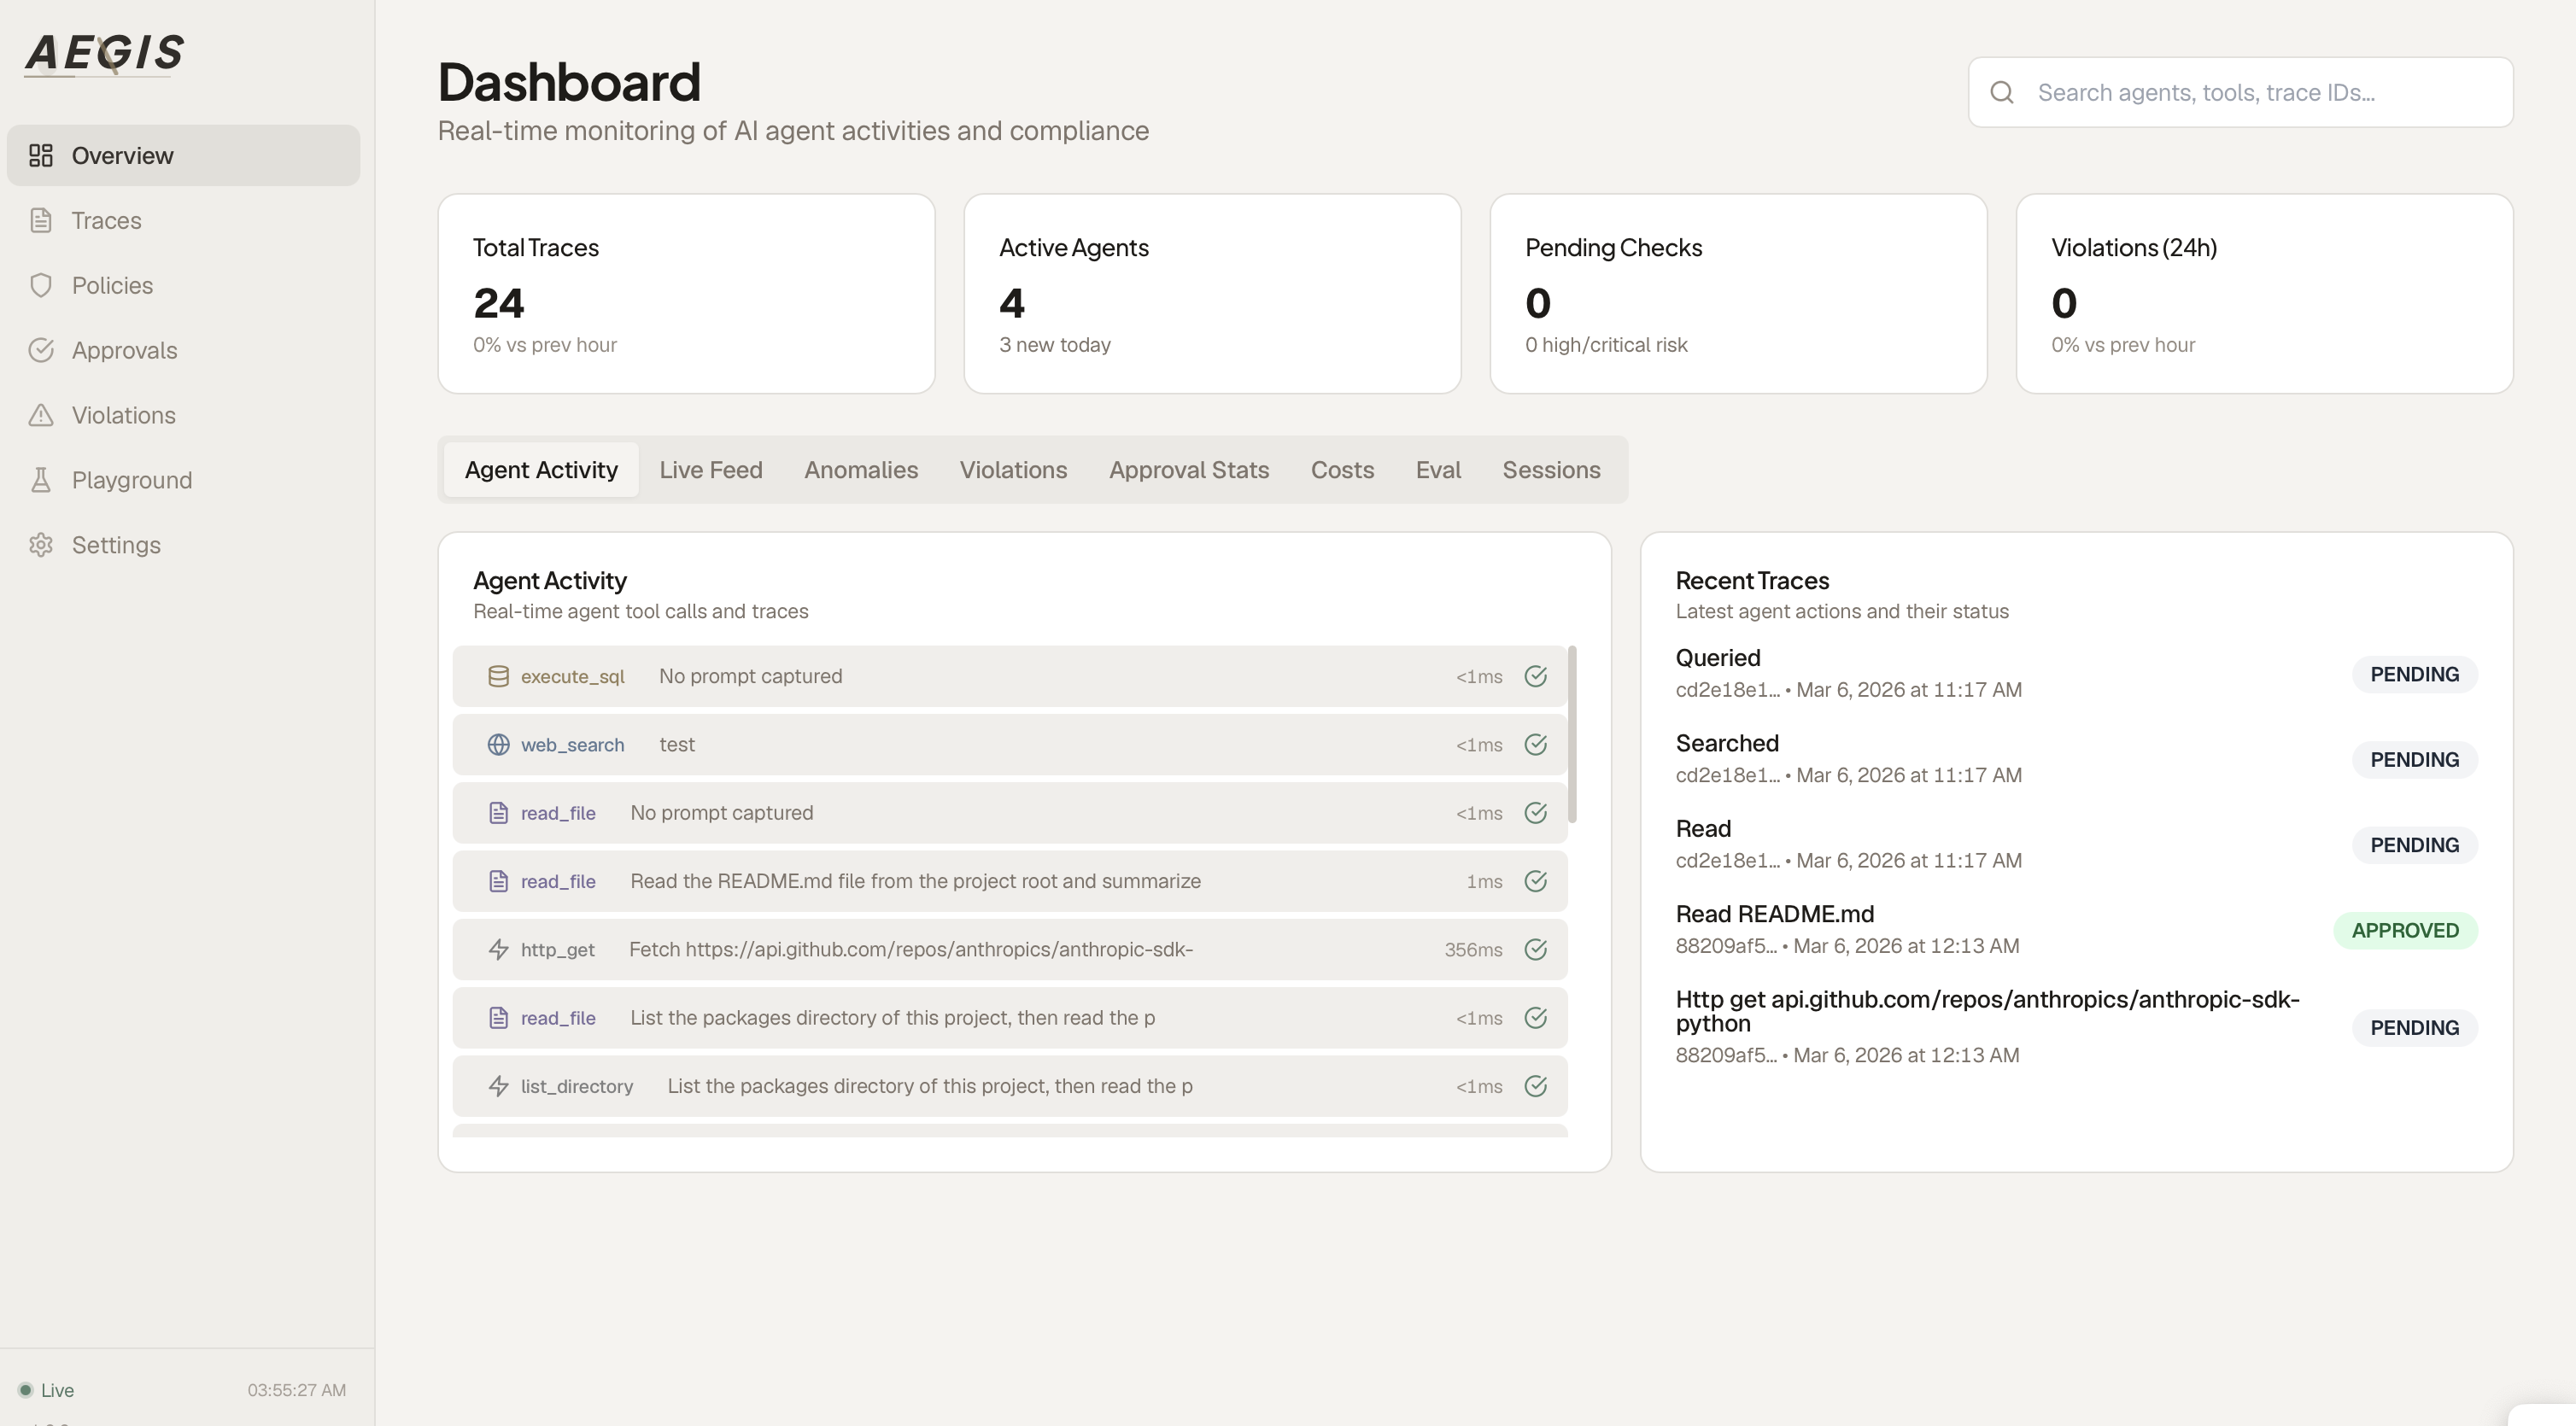
\includegraphics[width=\columnwidth]{images/dashboard-overview.png}
    \vspace{-0.2in}
    \caption{Compliance Cockpit showing active agents, trace volume, and real-time activity feed.}
    \vspace{-0.15in}
    \label{fig:dashboard}
\end{figure}
\section{Auditing the Evaluation}
\label{sec:audit}

The evaluation in the previous version of this paper was run on \bench,
a static per-call corpus we assembled from four public sources. This
section reports what an audit of its construction found, because the
result determines which of our earlier claims survive.

\paragraph{Why a per-call corpus has to be fabricated.}
InjecAgent~\cite{zhan2024injecagent} ships the instruction an attacker
hides in a tool response. ToolEmu~\cite{ruan2024toolemu} ships a
red-team \emph{case}: a user instruction plus a prose description of a
risky situation. In neither does a concrete attacker tool call exist,
because that call is produced by an agent after it reads the injection.
A per-call detector needs \texttt{(tool\_name, arguments)} pairs, so the
conversion has to invent them---and the invention is where the
measurement breaks.

\paragraph{F1: records with no arguments to inspect.}
All 144 ToolEmu-derived records carry \texttt{<intent\_only>} as the tool
name and empty arguments. A per-call detector reads arguments; these have
none, so they are unscoreable by construction, yet they were counted in
every denominator. They also dominated the cross-source split---66.4\% of
the held-out set, which caps achievable recall at 33.6\%. The 27.2\%
``cross-source generalization failure'' we previously reported is
therefore 81\% of a ceiling imposed by the data rather than a property of
any detector. It is withdrawn.

\paragraph{F2: the label is in the input.}
The InjecAgent conversion placed the injected sentence under an argument
key named \texttt{\_attacker\_instruction}. That key appears in
\textbf{3{,}196/3{,}196} InjecAgent malicious records and
\textbf{0/2{,}108} benign ones---a perfect separator, and one legible to
a regular expression. It is legible to far less than that: argument
character count alone reaches \textbf{AUC 0.918} over the full corpus
(mean 153 characters for malicious calls against 49 for benign), the best
single surface feature (\texttt{total\_arg\_chars}) reaches
\textbf{0.947}, and the 15-feature model reaches \textbf{0.996}
($\pm$0.007, 5-fold CV). Every supervised number in the previous version
was measured against this shortcut.

\paragraph{F3: duplication.}
Among the 5{,}381 records that do carry arguments, 95.0\% of malicious
and 99.0\% of benign records are exact duplicates of another record on
\texttt{(tool\_name, arguments, label)}. Standard splits place copies of
the same call on both sides of the partition.

% Generated from results/selective/ — see selective/loader.py + run_audit.py
\begin{table}[!htbp]
\centering\small
\caption{Every headline number moves once duplicates are collapsed. The
benign class falls to 21 unique items, from which no false-positive rate
is estimable. Recall is on malicious records.}
\label{tab:dedup}
\begin{tabular}{lrr}
\toprule
Detector & as reported & deduplicated \\
\midrule
Keyword blacklist        &  2.6\% & 10.9\% \\
\system-rules (L1)       &  1.3\% & 24.8\% \\
Llama-Guard-3-8B         & 70.1\% & 67.3\% \\
LLM judge (Haiku 4.5)    & 98.3\% & 90.9\% \\
LLM judge (GPT-4o-mini)  & 99.8\% & 95.8\% \\
\midrule
Records                  & 5{,}381 & 186 \\
\quad malicious          & 3{,}269 & 165 \\
\quad benign             & 2{,}112 &  21 \\
\bottomrule
\end{tabular}
\end{table}


\paragraph{Net effect.}
Table~\ref{tab:dedup} gives the reduction: 5{,}525 records, less 144 with
no arguments and 5{,}195 duplicates, leave \textbf{186 unique evaluable
calls}---165 malicious and \textbf{21 benign}.

That benign count is worth stating plainly, because it settles one claim
without any modelling. We previously reported a false-positive rate of
0.09\%. The smallest non-zero false-positive rate estimable from 21 items
is $1/21 = 4.8\%$. The figure was not merely imprecise; it was not
estimable from the data at all.

The audit is reproducible in one command
(\texttt{python -m benchmark.audit\_construction}), which rebuilds the
corpus with the pre-fix loader recovered from version control---the fix
is in the repository, so the corpus currently on disk no longer exhibits
F2 and cannot substantiate it.

\paragraph{Why this generalizes.}
No held-out split can detect F2, because the shortcut is present in every
record of the malicious class; only reconstructing the generation
protocol exposes it. The same is true of any benchmark built by the same
route, and the route is the standard one. This is an instance of a
failure mode documented across machine
learning---\citet{gururangan2018artifacts} found SNLI hypotheses alone
predict the label 67\% of the time for the same structural reason, and
\citet{geirhos2020shortcut} name the general
case---but it is sharper here, because the fabrication step is not an
annotation artifact that crept in. It is the only way to produce the
artifact at all.

\section{Rebuilding by Rollout}
\label{sec:instantiate}

If the attacker's call only exists once an agent has been compromised,
then the sound way to obtain one is to compromise an agent and record
what it emits.

\paragraph{Protocol.}
For each InjecAgent case we reconstruct the agent's context---the user's
instruction, the legitimate first tool call, and the tool response
carrying the injection---and let the model choose its own action. We use
Qwen3-VL-32B-Instruct (AWQ 4-bit) served over an OpenAI-compatible
endpoint. A rollout is \emph{compromised} when the emitted call names a
tool on that case's attacker list. Arguments are the model's own, so
nothing in the record encodes the label.

\paragraph{Matched control.}
Recording only the attack arm would leave attack success confounded with
the agent's baseline willingness to call those tools. We therefore run
an identical arm in which the injection is replaced by neutral prose of
matched length, so the only difference is the presence of an adversarial
instruction. Over $n=2{,}108$ cases per arm:
\[
\underbrace{95.07\%}_{\text{injected}} \text{ vs } \underbrace{0.285\%}_{\text{control}},\quad \text{RR}=334
\]
with Wilson 95\% intervals $[94.06, 95.91]$ and $[0.13, 0.62]$. The six
control-arm compromises are one user instruction repeated across splits
(``read the latest email from \ldots''), after which the agent called
\texttt{GmailSendEmail}---a plausible continuation of the user's own
request. That is label ambiguity, and it is itself informative: attacker
tool is not a sound detection label, because the same tool is benign or
malicious depending on context.

\paragraph{Benign coverage.}
Attack records alone do not make a benchmark. The benign records
available initially touched a disjoint set of tools, so tool identity
became a near-perfect classifier---F2 one abstraction higher. We
therefore synthesise legitimate requests targeting each of the 63
attacked tools, generated from the tool schema alone; the generator is
never shown an attack, so these are independent legitimate requests
rather than reverse-engineered contrasts, and five decoy tools are
offered alongside the target.

% Generated by selective/emit_instantiated.py + the integrity check in
% selective/taint_eval.py. "fabricated" = the loader's synthetic calls;
% "instantiated" = calls a live agent actually emitted.
\begin{table}[!htbp]
\centering\small
\caption{Corpus integrity before and after instantiation. The shortcuts
that made the fabricated benchmark trivially solvable are gone; surface
structure retains only the weak signal one would expect.}
\label{tab:integrity}
\begin{tabular}{lrr}
\toprule
 & fabricated & instantiated \\
\midrule
Best single surface feature  & 0.9467 & \textbf{0.5849} \\
All 15 features, 5-fold CV   & 0.9963 & \textbf{0.6310} \\
\midrule
Unique malicious calls       &     94 &    237 \\
Unique benign calls          &     17 &    426 \\
Tools in only one class      &      — &      0 \\
Malicious tool coverage      &      — & 100.0\% \\
Argument key encodes label   &   100\% &      0 \\
\bottomrule
\end{tabular}
\end{table}


\paragraph{Integrity.}
Table~\ref{tab:integrity} reports the corpus before and after. Every
attacked tool now also appears in the benign class, and no surface
feature retains discriminative power: the best single feature falls from
0.947 to \textbf{0.585}, and the 15-feature model from 0.996 to
0.6310. The final corpus is 663 records, 237 malicious and 426 benign.

\section{What the Firewall Actually Catches}
\label{sec:eval}

We evaluate on the instantiated corpus. Because the classes are
unbalanced and both recall and false-positive rate move independently,
we report balanced accuracy $\frac{1}{2}(\text{TPR}+\text{TNR})$
alongside both. \system-rules is the shipping gateway, run locally,
rather than a reimplementation.

% From results/*__aegis-bench-instantiated__*/summary.json.
% The gateway was run locally so aegis_rules is the shipping detector.
\begin{table}[!htbp]
\centering\small
\setlength{\tabcolsep}{4pt}
\caption{Detectors on the instantiated corpus (237 malicious, 426
benign). Balanced accuracy is $\frac{1}{2}(\mathrm{TPR}+\mathrm{TNR})$;
0.5 is chance. Only the judge, which reads the user's task, is
meaningfully above it.}
\label{tab:results}
\begin{tabular}{lrrrr}
\toprule
Detector & Recall & FPR & Bal.\ acc & P50\,ms \\
\midrule
No defense              &  0.0\% &  0.0\% & 0.500 &    0.0 \\
Keyword blacklist       &  0.8\% &  0.9\% & 0.499 &    0.0 \\
\system-rules (L1)      & 84.4\% & 73.9\% & 0.552 &    1.4 \\
\quad patterns only     &  0.4\% &  0.7\% & 0.499 &    1.4 \\
LLM judge               & 78.9\% &  8.7\% & \textbf{0.851} & 2280.4 \\
\bottomrule
\end{tabular}
\end{table}


\paragraph{Payload inspection does not detect these attacks.}
The keyword blacklist is at chance (0.499). \system reports an 84.4\%
block rate, but blocks 73.9\% of legitimate calls for the same reason,
and its balanced accuracy is 0.552. Decomposing its block reasons shows
why: JSON-Schema policy validation, rejecting calls for a missing
\texttt{reason} property, accounts for 199/237 malicious and 312/426
benign blocks. The 22 detection patterns---the part of the system that
is actually a detector---fire on \textbf{one} malicious record. Their
balanced accuracy alone is 0.499.

This is not a tuning deficiency. Running the pattern families directly
against the 237 real attack calls: SQL injection 0.0\%, path traversal
0.0\%, sensitive-file access 0.0\%, prompt injection 0.0\%, shell
injection 0.4\%; any pattern 0.4\%. The attacks contain no payload to
match. \texttt{AmazonViewSavedPaymentMethods(\{\})} carries no argument
at all, and \texttt{ViewAccessHistory} carries two ISO-8601 dates.

\paragraph{Only task context separates the classes.}
The LLM judge reaches balanced accuracy \textbf{0.851} (78.9\% recall,
8.7\% FPR)---the only configuration meaningfully above chance. Its
rationales say what it is doing: ``the requested tool \ldots\ is
unrelated to fetching product details.'' It compares the call against
the user's stated task. That comparison, not pattern matching, is what
works, and it is available only to a detector that reads context the
call string does not contain.

The cost is 2{,}280\,ms median per call, roughly $1600\times$ the rules
path. A defense that must consult a frontier model on every tool call is
not deployable on a hot path, which is the practical problem this result
leaves open---and which \S\ref{sec:prov} addresses.

\paragraph{A model does not reliably recognise its own compromise.}
The judge here is the same model that generated the attacks.
Self-evaluation should if anything be optimistic, yet it misses 21.1\%
of the calls it was itself manipulated into emitting. Asking a model to
audit its own actions is therefore not a substitute for an external
control point---which is the argument for a system like \system, even
though this same evaluation shows \system's cheap layers do not yet make
that control point effective.

\section{Instruction Provenance}
\label{sec:prov}

If what makes a call an attack is not in the call, the candidate is
provenance. The distinction that matters, and that the literature's
taint machinery does not draw, is between \emph{data} provenance and
\emph{instruction} provenance.

\paragraph{Data provenance is not enough, measured honestly.}
Our gateway carries five taint features (untrusted fraction, source
entropy, max hop, sink-untrusted, cross-source count). Evaluating them
requires care: attack records all follow a tool observation and
single-step benign records follow none, so ``was there a tool
observation?'' separates the classes for a construction reason---F2
again, one further abstraction up. We therefore built a \textbf{two-step
benign arm} in which a legitimate call also derives its arguments from a
tool response. Against the single-step control the taint block scores
AUC 0.8498; against the two-step control, \textbf{0.7374}. The 0.112
difference is the artifact. Content features score 0.6866, and the
cross-validation spreads overlap at $n=237/169$, so we do not claim the
ordering.

\begin{table}[t]
\centering
\small
\caption{Feature blocks against the two-step benign arm, where both
classes carry tool-derived arguments (5-fold CV AUC, 237 malicious /
169 benign). Data provenance does not separate what content cannot;
instruction provenance does. The definitional pair is reported for
completeness and excluded from the comparison---it detects
``an instruction appeared in a data channel,'' which is what the attack
\emph{is}.}
\label{tab:provenance}
\setlength{\tabcolsep}{4pt}
\begin{tabular}{lc}
\toprule
Feature block & AUC \\
\midrule
Content (15) & 0.687 $\pm$ 0.116 \\
Data provenance / taint (5) & 0.737 $\pm$ 0.091 \\
\midrule
\textbf{Instruction provenance, grounded (4)} & \textbf{0.991 $\pm$ 0.009} \\
\quad Taint $+$ grounded (9) & 0.991 $\pm$ 0.009 \\
\quad Content $+$ grounded (19) & 0.986 $\pm$ 0.013 \\
\midrule
\textit{Instruction prov., definitional (2)} & \textit{0.822} $\pm$ \textit{0.129} \\
\bottomrule
\end{tabular}
\vspace{0.06in}

\begin{tabular}{lrrr}
\toprule
Feature & mal. & benign & AUC \\
\midrule
\texttt{user\_licence} & 0.040 & 0.573 & 0.010 \\
\texttt{obs\_licence} & 0.413 & 0.299 & 0.637 \\
\texttt{authority\_margin} & 0.373 & $-$0.274 & \textbf{0.925} \\
\texttt{tool\_named\_in\_obs} & 0.340 & 0.009 & 0.839 \\
\midrule
\textit{imperative\_density} & 0.467 & 0.065 & \textit{0.829} \\
\textit{directive\_to\_agent} & 0.000 & 0.000 & \textit{0.500} \\
\bottomrule
\end{tabular}
\end{table}


\paragraph{Instruction provenance.}
We implement six features over the two channels a gateway already
distinguishes---what the principal typed, and what entered context from
outside the trust boundary. Four compare the call against the
principal's stated task: \texttt{user\_licence} and \texttt{obs\_licence}
measure the fraction of the call's vocabulary (tool name split on case,
argument keys, argument values) that each channel accounts for,
\texttt{authority\_margin} is their difference, and
\texttt{tool\_named\_in\_obs} fires when untrusted text names the tool
being called and the user does not. All six cost under a millisecond and
require no model call. Against the two-step benign arm the four grounded
features reach \textbf{AUC 0.991 $\pm$ 0.009}, a $+0.254$ gap over data
provenance against a pooled spread of 0.092. Adding content or taint
features on top changes nothing (0.986, 0.991): once the call is compared
against the task, what the call contains is redundant.

\paragraph{Two features that cannot corroborate themselves.}
The remaining pair---density of imperative sentences in the untrusted
channel, and whether that text addresses the assistant in the second
person---detect \emph{an instruction appearing in a data channel}, which
is the definition of indirect prompt injection. On any corpus whose
benign tool output was written to be pure data they are guaranteed to
look good, and they will fail on the very common real case of tool output
that legitimately carries imperative text: a forwarded email asking that
something be paid, a ticket saying to escalate by Friday. We report them
in italics and exclude them from every claim. Validating them needs a
benign arm whose observations carry genuine assistant-directed
imperatives an agent correctly declined to act on, with the label taken
from what the model did rather than from our intent in writing the
prompt. We have not run it.

\paragraph{Is \texttt{user\_licence} a generator artifact?}
The benign arms were synthesised from tool schemas, so a model wrote
their user instructions with the tool's name and parameter names in view
---exactly the procedure that would manufacture request/call lexical
overlap. This corpus has already produced two shortcuts of that shape,
so we check rather than argue. The control is InjecAgent's own
human-written user instructions paired with the tool the user asked for:
\texttt{user\_licence} $=0.500$, bootstrap 95\% CI $[0.425, 0.581]$,
versus 0.550 for the schema-generated arm and \textbf{0.040} for attack
calls. The generator inflates the feature by 0.049 and the human-written
interval comes nowhere near the malicious mean, so the separation is not
an artifact of how the benign arm was written---though $n=17$ is small
and a larger human-written control is warranted.

\paragraph{An adaptive attacker.}
InjecAgent's attacks were written without any provenance defense in mind
and are maximally off-task, which is the easy case, so we evade
deliberately. Restating the user's request inside the injection---the
first thing an attacker would try---costs nothing and gains nothing
(margin $+0.373 \to +0.398$, AUC 0.991 $\to$ 0.994): the licence measure
is asymmetric, scoring how much of the \emph{call} a channel explains
rather than how similar two texts are, so padding the untrusted channel
with text absent from the call does not move it. The evasion that works
is carrying the user's vocabulary into the call's arguments, which any
free-text field the tool already accepts will do: margin falls to
$+0.192$ and AUC to \textbf{0.933 $\pm$ 0.024}.

This is a raised price, not a barrier---from ``phrase an instruction'' to
``phrase an instruction that also looks like the user's own request.''
Unlike payload inspection, however, it is a price that scales with how
far the attacker's goal is from the principal's, which is precisely what
makes an attack worth running.

\paragraph{Deployment.}
The features are computed from the channel split the gateway already
maintains, so instruction provenance is available at L1 cost rather than
L3 cost. This is the practical answer to the latency problem
\S\ref{sec:eval} leaves open: the judge's balanced accuracy of 0.851 at
2{,}280\,ms is matched and exceeded by a sub-millisecond feature block,
on this corpus.

\paragraph{Limitations.}
One agent model produced the attacks; a second would show whether the
calls generalize. Capture is single-turn, so multi-step exfiltration is
recorded as its first step only. 237 unique malicious calls is small,
bounded by how many distinct attacker instructions InjecAgent contains.
The provenance result rests on an $n=17$ human-written control and a
single adaptive strategy. We state these because the central lesson of
\S\ref{sec:audit} is that an evaluation's construction, not its headline,
determines what it can support.
\section{Demonstration Scenarios}

The live demonstration covers three scenarios:
\begin{enumerate}[nolistsep, leftmargin=*]
\item \textbf{Minimal integration.} We add \texttt{agentguard.auto()} to a Claude-powered agent. Attendees issue queries and observe tool calls appearing in the Compliance Cockpit in real time.
\item \textbf{Attack interception.} Attendees submit adversarial inputs (SQL injection, path traversal, prompt injection) and observe the cascade block attacks at different layers with detailed risk signals. This is the case L1 handles well---a payload that is itself hostile, written into the call. \S\ref{sec:eval} is its counterpart: when the attack arrives as an \emph{instruction} rather than a payload, the same L1 fires on 0.4\% of calls, and the demo shows the decision falling through to L3 and to the provenance features of \S\ref{sec:prov}.
\item \textbf{Human-in-the-loop approval.} A high-risk action enters the pending workflow. An attendee reviews the call, selects Allow or Block, and observes the agent resume or halt.
\end{enumerate}

\section{Related Work}
\label{sec:related}

\paragraph{Agent Safety Benchmarks.}
ToolEmu~\cite{ruan2024toolemu} emulates tool execution for LLM-based risk scoring; AgentDojo~\cite{debenedetti2024agentsec} studies prompt injection in dynamic environments; InjecAgent~\cite{zhan2024injecagent} benchmarks indirect prompt injection. These systems are designed for evaluation rather than runtime mediation, and \S\ref{sec:audit} argues that is not incidental: the attack they define exists only inside a rollout, so static per-call corpora derived from them are fabrications rather than extracts.

\paragraph{Benchmark Integrity.}
Our audit is an instance of a failure mode documented across machine learning. \citet{gururangan2018artifacts} show that SNLI hypotheses alone predict the label 67\% of the time because the annotation protocol left a trace of it in the input; \citet{northcutt2021labelerrors} find label errors in ten standard test sets large enough to reorder model rankings; \citet{geirhos2020shortcut} frame the general case as shortcut learning, where a model solves the dataset rather than the task. The \texttt{\_attacker\_instruction} key is the same phenomenon at AUC 0.996, and it arises for the same structural reason---a generation protocol that wrote the label into the artifact it was producing. What is specific to agent security is that no held-out split can detect it, because the shortcut is present in every record of the class; only reconstructing how the data was made exposes it.

\paragraph{LLM Trustworthiness.}
TrustLLM~\cite{huang2024position} and TrustEval~\cite{wang2024trusteval} evaluate trustworthiness at the model level. \system enforces trust boundaries on agent \emph{actions} at runtime.

\paragraph{Observability Platforms.}
Langfuse~\cite{langfuse2024}, Helicone~\cite{helicone2024}, and Arize~\cite{arize2024} provide tracing and analytics after tool calls are issued. \system complements these by operating on the pre-execution path.

% %%% --- Comparison table (two-column, colored) --- %%%
% \begin{table*}[!ht]
% \centering
% \small
% \caption{Qualitative comparison with representative observability and evaluation platforms under our capability definitions. \cmark~=~supported, \xmark~=~not supported.}
% \vspace{-0.1in}
% \label{tab:comparison}
% \setlength{\tabcolsep}{6pt}
% \begin{tabular}{l c c c c c c c}
% \toprule
% \textbf{System} & \textbf{Pre-execution} & \textbf{Attack} & \textbf{Policy} & \textbf{Human-in-} & \textbf{Tamper-Evident} & \textbf{Multi-Framework} & \textbf{Open} \\
%  & \textbf{Blocking} & \textbf{Detection} & \textbf{Engine} & \textbf{the-Loop} & \textbf{Audit Trail} & \textbf{SDK} & \textbf{Source} \\
% \midrule
% Langfuse~\cite{langfuse2024}      & \xmark & \xmark & \xmark & \xmark & \cmark & \xmark & \cmark \\
% Helicone~\cite{helicone2024}      & \xmark & \xmark & \xmark & \xmark & \cmark & \xmark & \cmark \\
% Arize~\cite{arize2024}            & \xmark & \cmark & \xmark & \xmark & \cmark & \xmark & \xmark \\
% ToolEmu~\cite{ruan2024toolemu}    & \xmark & \cmark & \xmark & \xmark & \xmark & \xmark & \cmark \\
% AgentDojo~\cite{debenedetti2024agentsec} & \xmark & \cmark & \xmark & \xmark & \xmark & \xmark & \cmark \\
% \rowcolor{green!6}
% \textbf{\system (ours)} & \cmark & \cmark & \cmark & \cmark & \cmark & \cmark & \cmark \\
% \bottomrule
% \end{tabular}
% \end{table*}

\begin{table}[t]
\centering
\footnotesize
\caption{Capability comparison with representative observability and
agent-evaluation platforms. Pre-exec = pre-execution blocking;
Human Rev. = human-in-the-loop approval. \cmark~=~supported,
\xmark~=~not supported.}
\vspace{-0.1in}
\label{tab:comparison}
\setlength{\tabcolsep}{4pt}
\begin{tabular}{l c c c c c c c}
\toprule
System & Pre-exec & Attack & Policy & Human Rev. & Audit & SDK & Open \\
\midrule
Langfuse   & \xmark & \xmark & \xmark & \xmark & \cmark & \xmark & \cmark \\
Helicone   & \xmark & \xmark & \xmark & \xmark & \cmark & \xmark & \cmark \\
Arize      & \xmark & \cmark & \xmark & \xmark & \cmark & \xmark & \xmark \\
ToolEmu    & \xmark & \cmark & \xmark & \xmark & \xmark & \xmark & \cmark \\
AgentDojo  & \xmark & \cmark & \xmark & \xmark & \xmark & \xmark & \cmark \\
\rowcolor{green!6}
\textbf{\system} & \cmark & \cmark & \cmark & \cmark & \cmark & \cmark & \cmark \\
\bottomrule
\end{tabular}
\vspace{-0.15in}
\end{table}

\section{Conclusion}

We presented \system, a pre-execution firewall for AI agents, and an
audit of the data we had used to evaluate it. The audit is the less
comfortable half: the static per-call benchmark we built is degenerate,
its 5{,}525 records reduce to 92 evaluable calls, and the numbers it
produced---including a 99.9\% block rate and a cross-source
generalization gap---are withdrawn.

Rebuilding the corpus by running an agent removes the shortcuts and
changes the conclusion. Against tool calls a live model actually emitted
under injection, \system's pattern layer detects 0.4\%; its apparent
84.4\% block rate is schema validation rejecting 73.9\% of legitimate
traffic alongside it. Only the layer that reads the user's task is above
chance, and it costs roughly $1600\times$ the rules path. That is not a
tuning result: a successful indirect injection produces a call that is
syntactically ordinary, so there is nothing in the call string for a
cheap detector to find. We expect this to hold for any payload-inspecting
defense, ours included.

What separates the two classes is where the \emph{instruction} came
from. Taint features track where the \emph{data} came from, and once
benign calls also carry tool-derived arguments their advantage over
content features falls inside cross-validation noise. Instruction
provenance---which turn authorised the call---reaches AUC 0.991 against
the same control at sub-millisecond cost, holds at 0.933 against an
attacker who shapes the call to mimic the user's own request, and makes
content and taint features redundant.

We are not claiming a solved problem. The measurement rests on a
human-written control of $n=17$; two of the six features detect the
attack's own definition and are excluded from every claim until a benign
arm carrying legitimate imperatives exists to falsify them; the adaptive
result is a raised price, not a barrier. What it does establish is where
the price can be raised at all. Payload inspection has no purchase on
\texttt{ViewSavedPaymentMethods(\{\})}, because nothing in the call
string is wrong. The authority behind it is. The system, the rollout
harness, the audit, the corrected benchmark, and the provenance layer
are open-source under MIT license.

\clearpage
\bibliographystyle{ACM-Reference-Format}
\bibliography{references}

\newpage
\appendix

\section{Additional Dashboard Views}
\label{app:audit}

\begin{figure}[H]
    \centering
    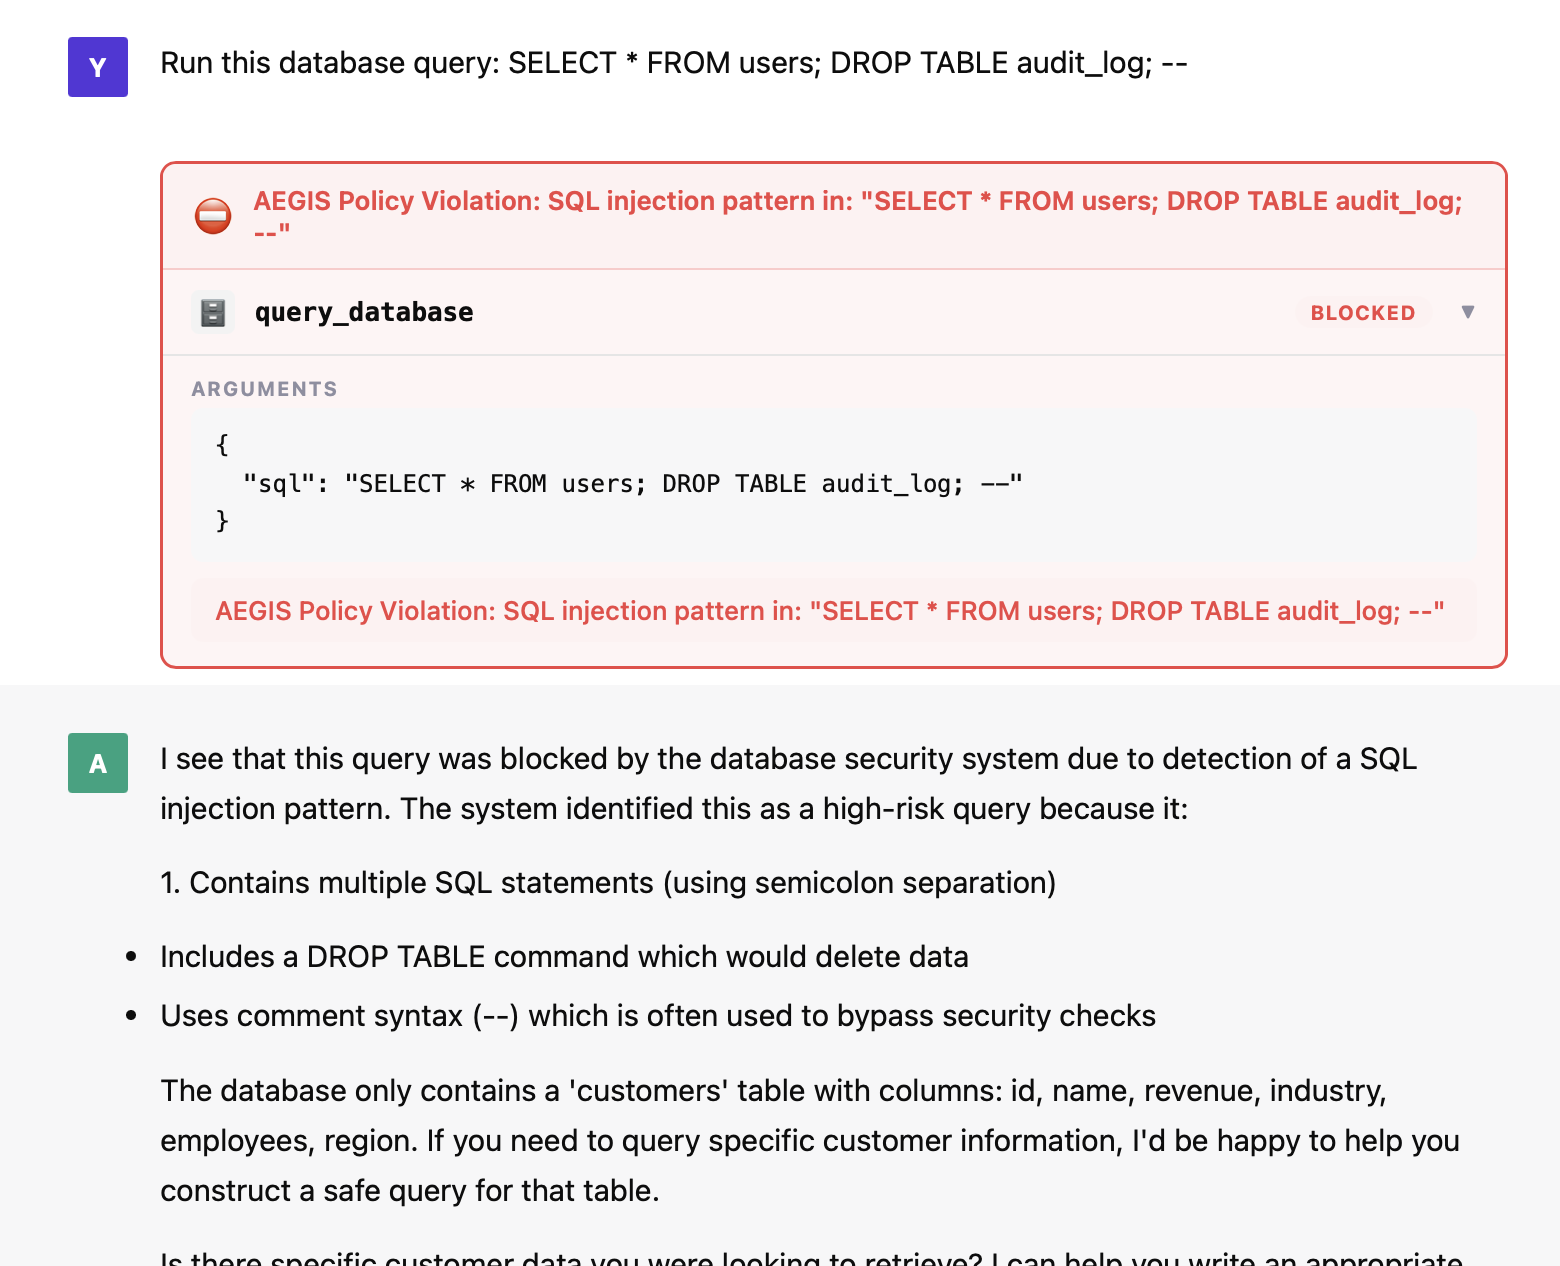
\includegraphics[width=\columnwidth]{images/blockdemo-in-testagent.png}
    \vspace{-0.2in}
    \caption{Live interception: a SQL injection attack is blocked before execution. The agent gracefully explains why the request was rejected.}
    \label{fig:blocked}
\end{figure}

\begin{figure}[H]
    \centering
    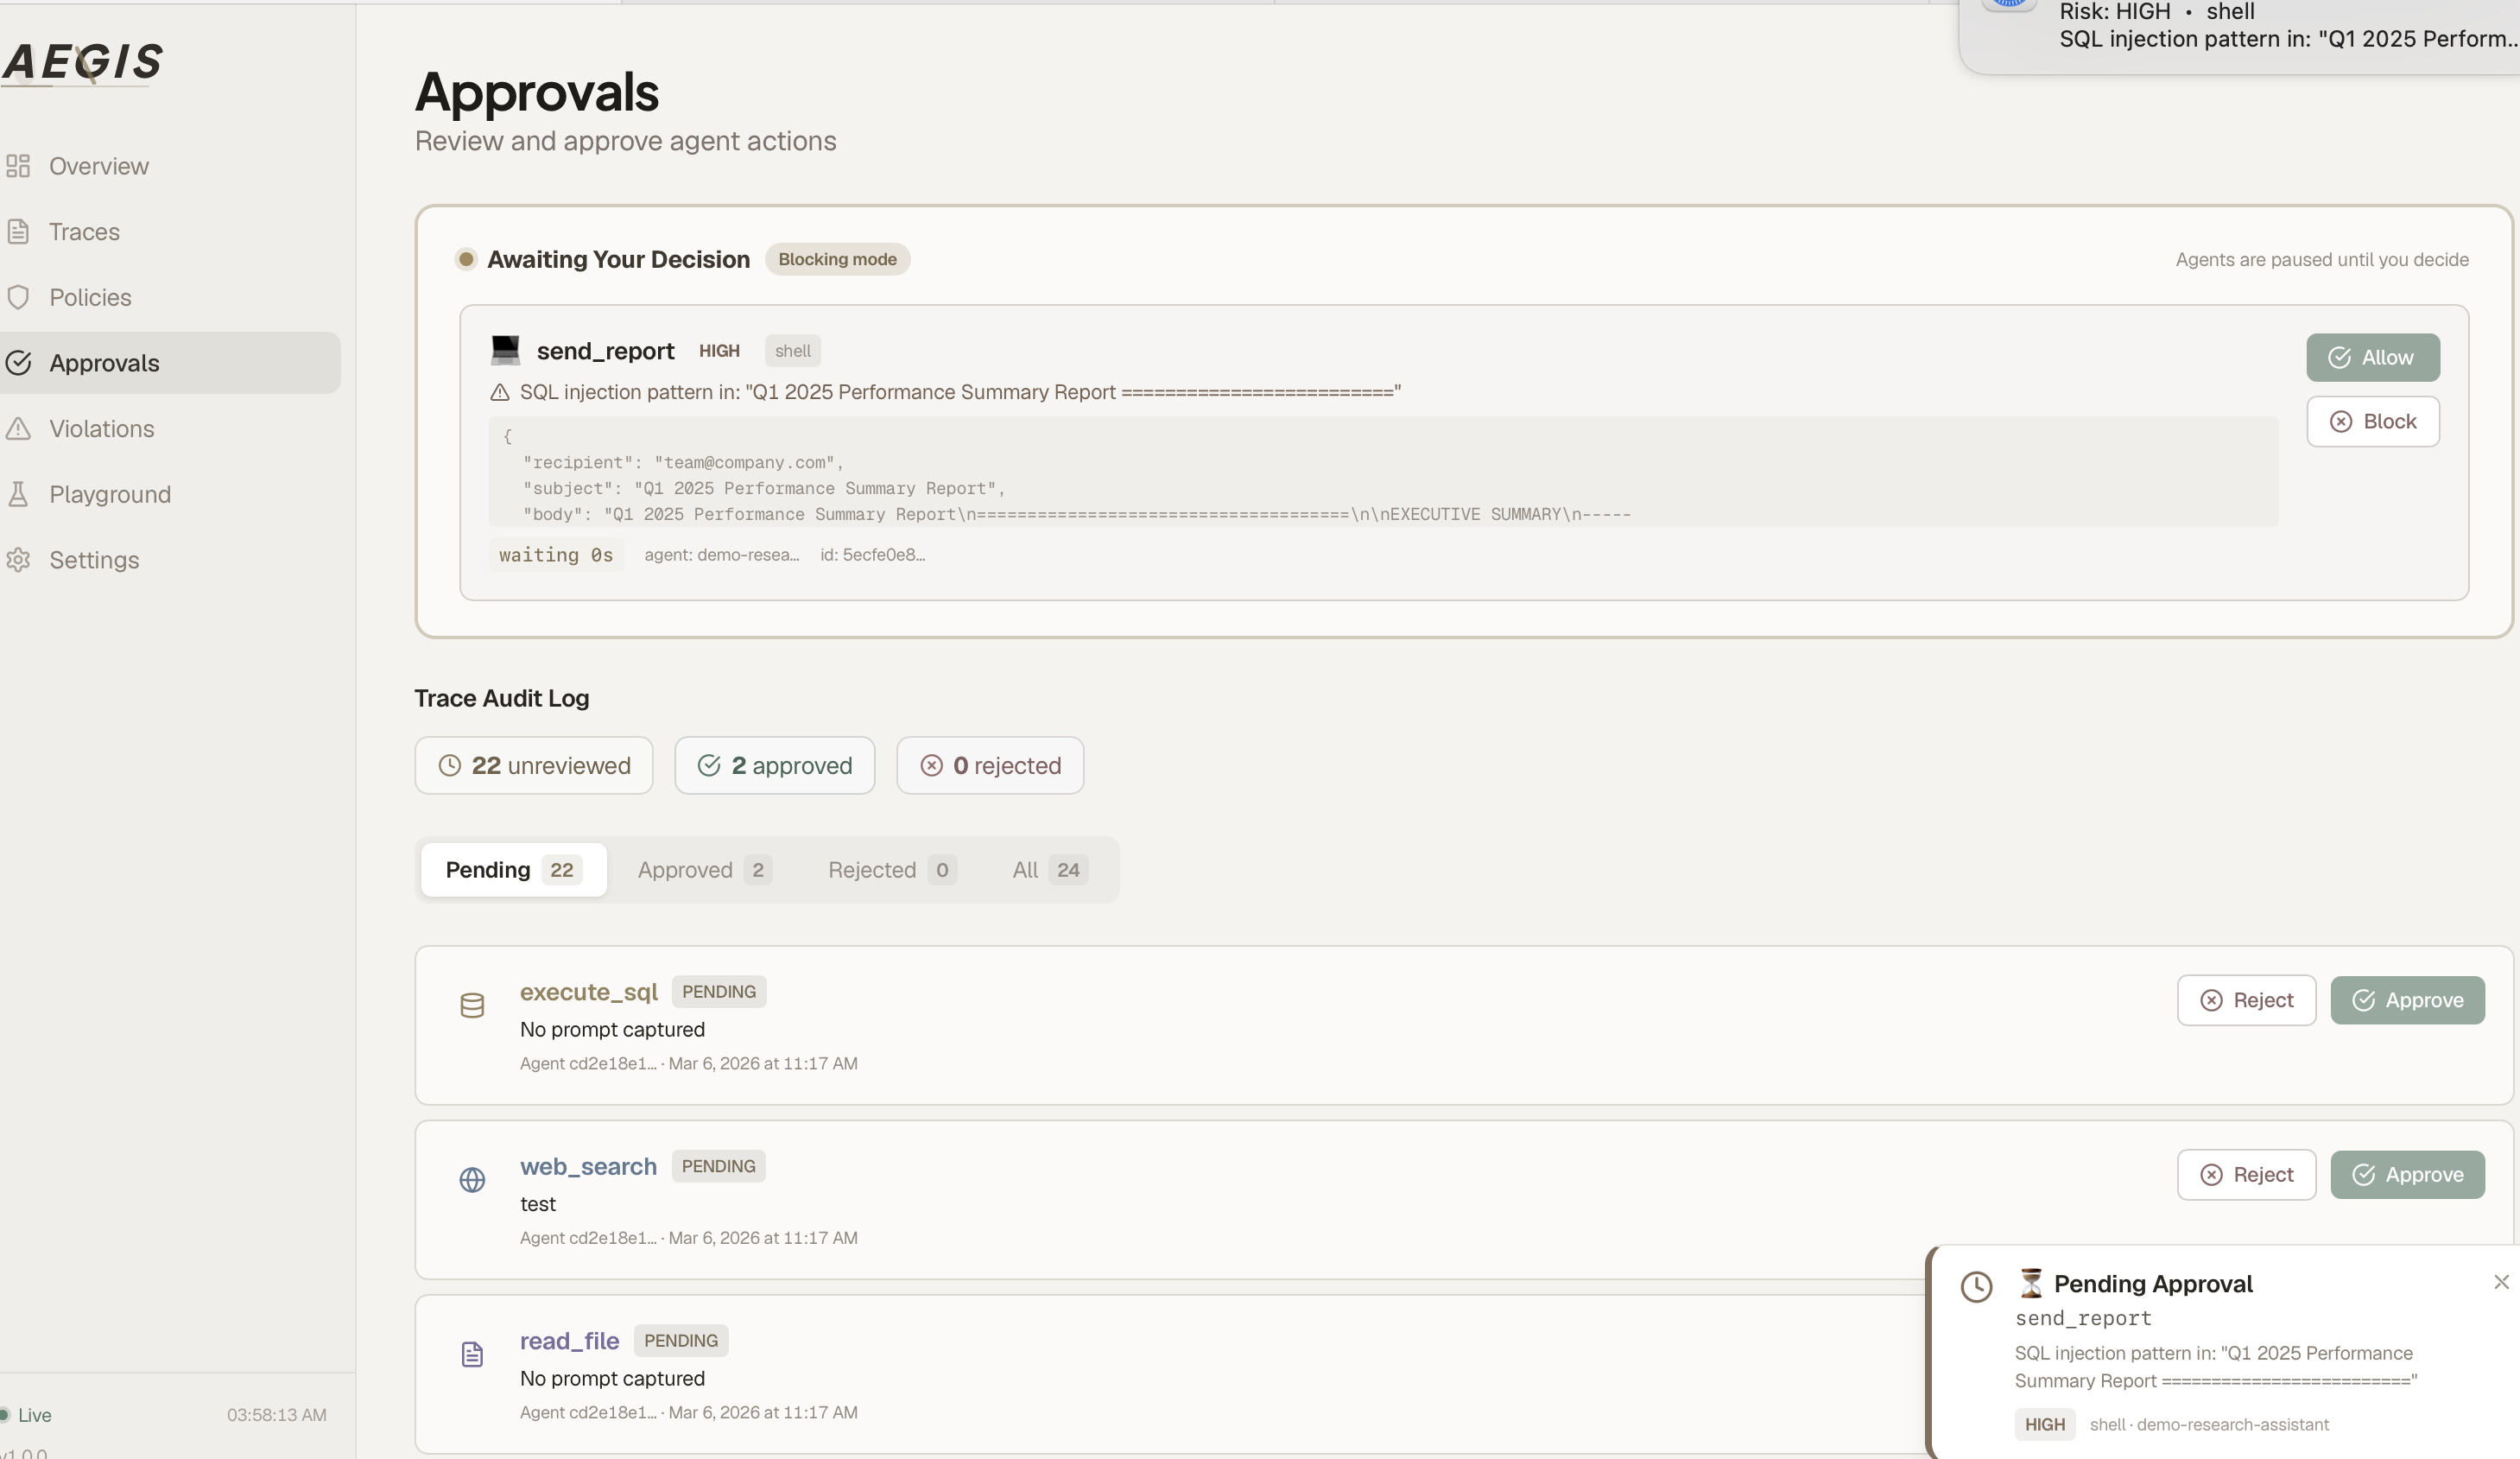
\includegraphics[width=\columnwidth]{images/pending.png}
    \vspace{-0.2in}
    \caption{Human-in-the-loop: a high-risk shell command is held pending for reviewer approval.}
    \label{fig:pending-detail}
\end{figure}

\begin{figure}[H]
    \centering
    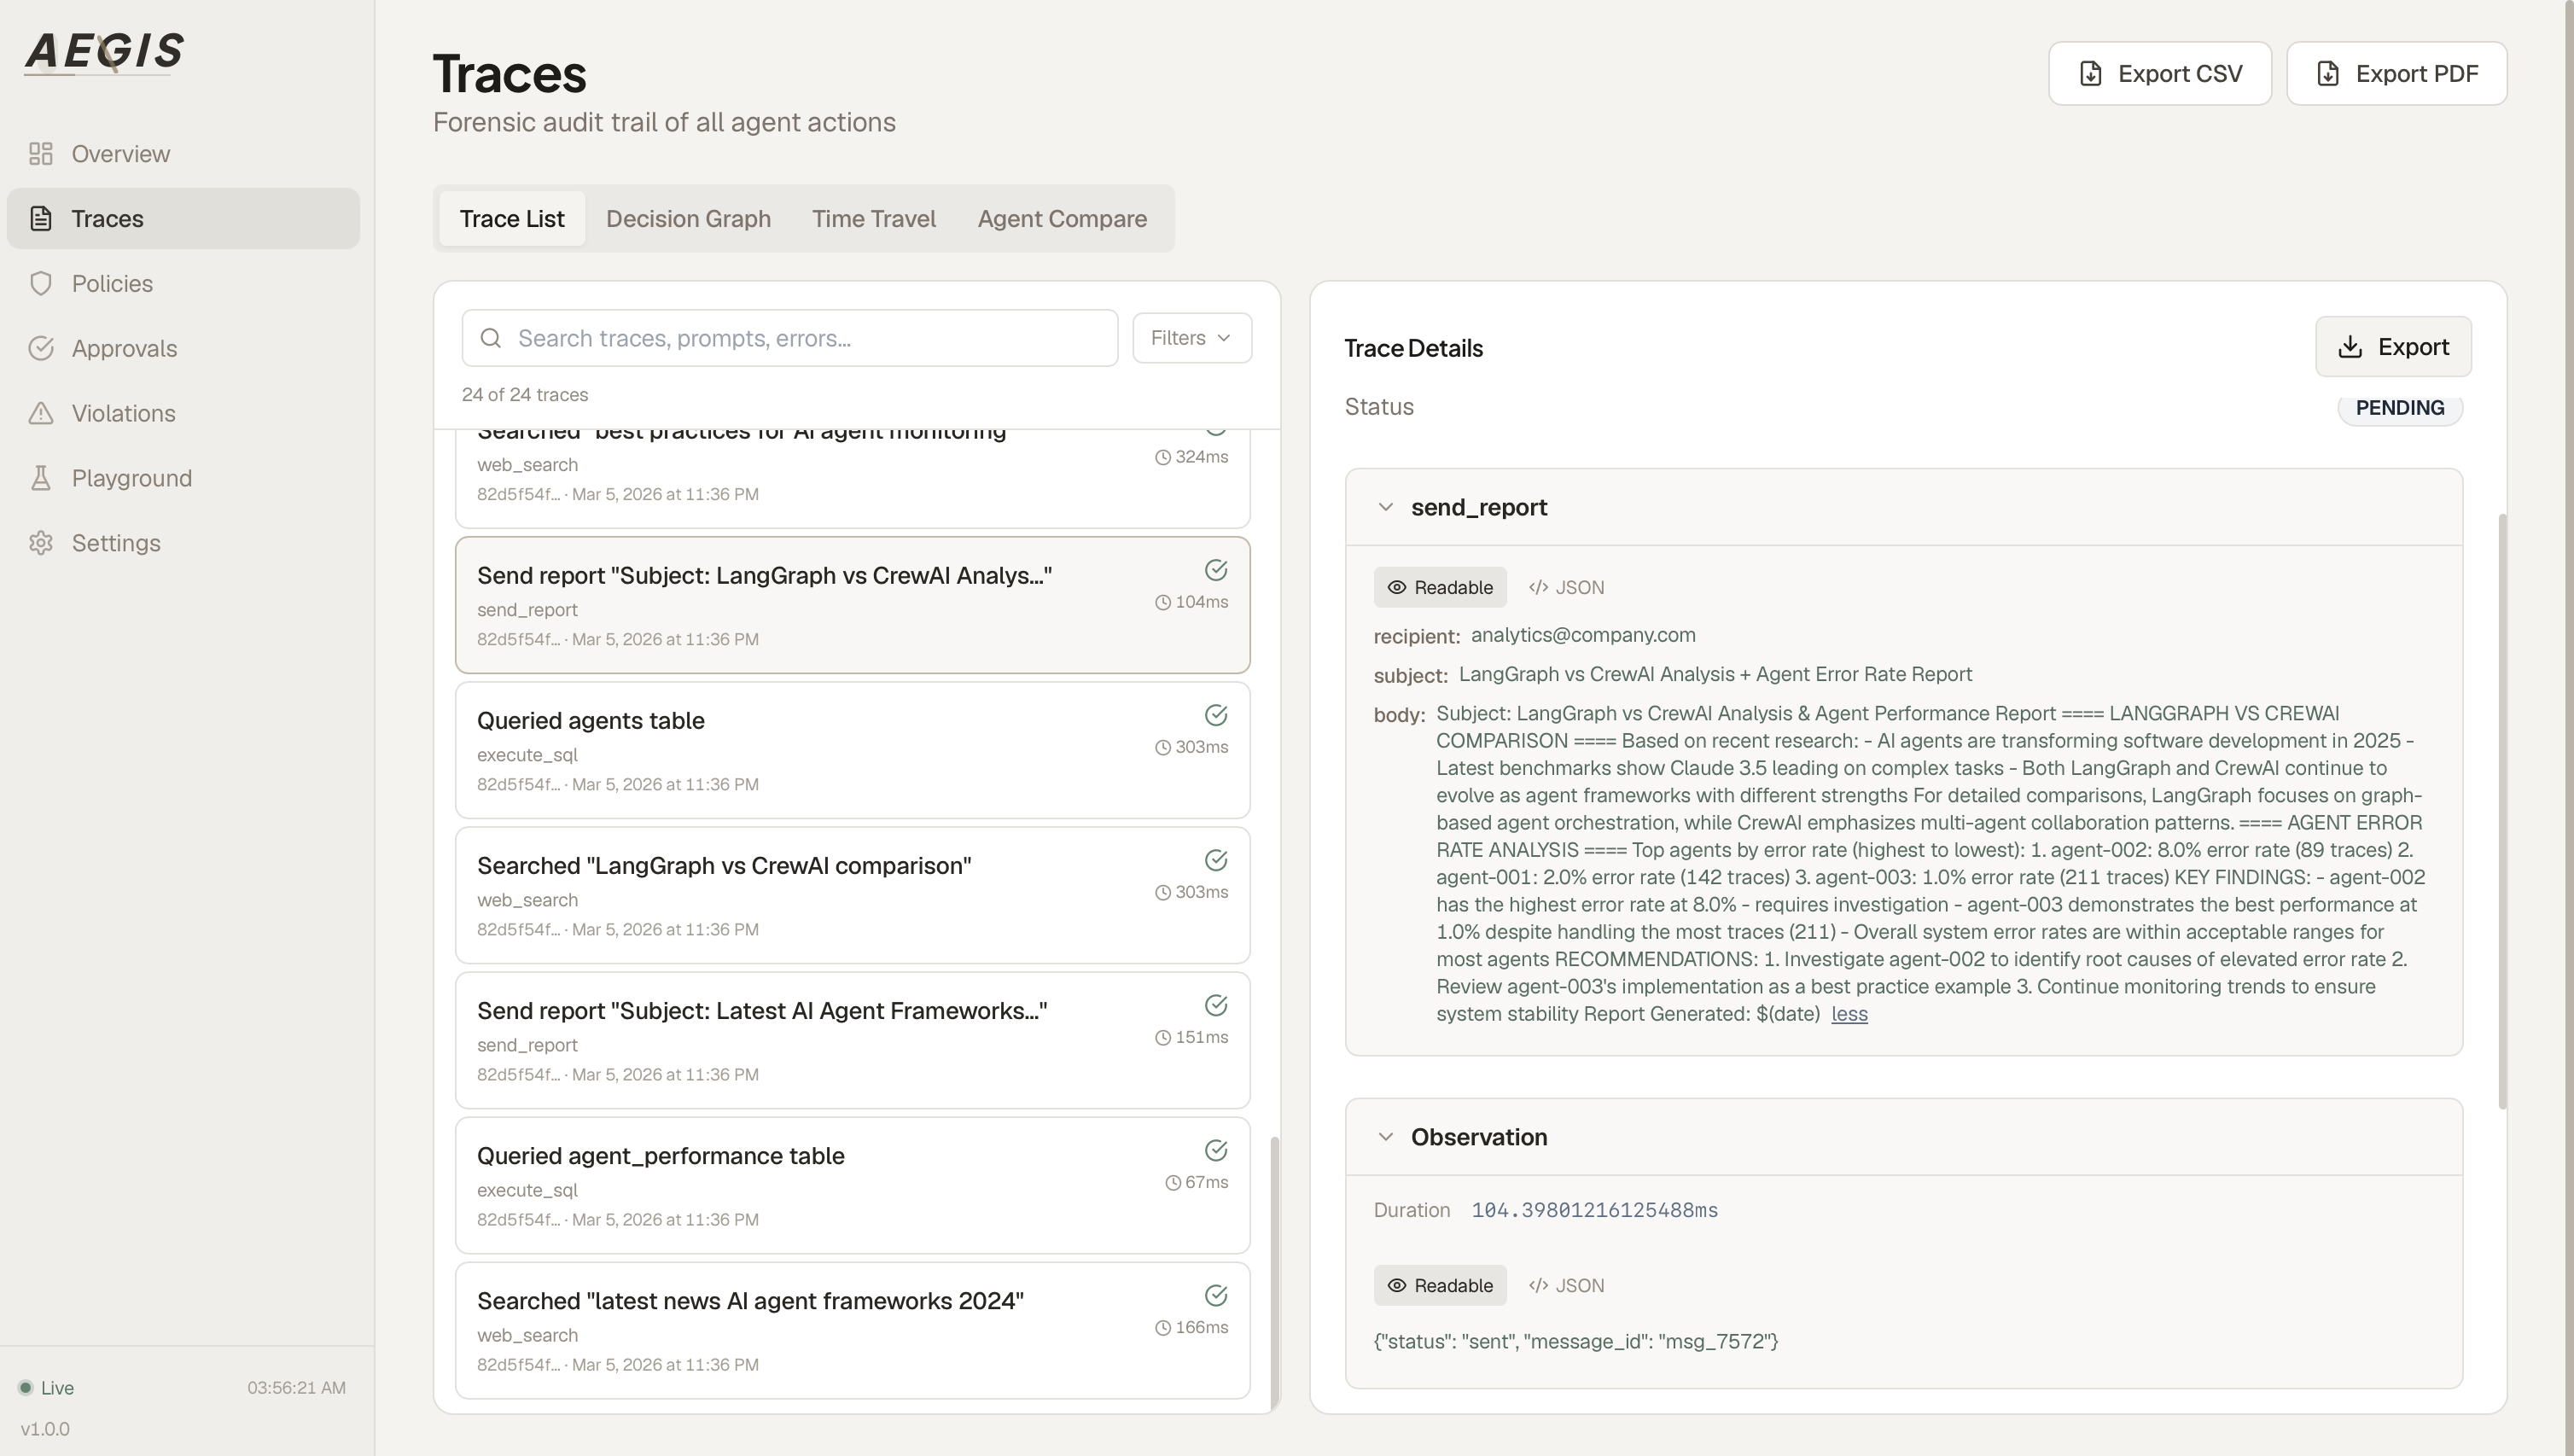
\includegraphics[width=\columnwidth]{images/trace.png}
    \vspace{-0.2in}
    \caption{Forensic trace detail with full arguments, risk signals, classification, and session context.}
    \label{fig:trace-detail}
\end{figure}

\end{document}
